
% Preamble
\documentclass[11pt]{article}

% Packages
\usepackage{amsmath}
\usepackage[letterpaper,margin=2cm]{geometry}
\usepackage[utf8]{inputenc}
\usepackage[spanish, english]{babel}
\usepackage{amssymb, amsmath, amsbsy, amsfonts}
\usepackage{upgreek}
\usepackage{graphicx}
\usepackage{multicol}
\usepackage{color}
\usepackage{caption}
%\usepackage[style=apa]{biblatex}
\renewcommand{\figurename}{Fig.}
\renewcommand{\tablename}{Tab.}
\setlength{\columnsep}{5mm}
\title{\textbf{Acá va el título del experimento}\\{\textcolor{red}{Acá va el apellido paterno, apellido materno y nombres\\Acá va el apellido paterno, apellido materno y nombres}}}
\author{LAB122A-XX-YY o B-XX-YY, Laboratorio de Física I, INF-FCPN-UMSA}
\date{\today}

% Document
\begin{document}
    \maketitle
    \selectlanguage{spanish}
    \begin{abstract}
        \noindent Es uno de los aspectos más importantes del informe. Describe de una forma tal que un lector reconoce los conceptos más sobre salientes del informe. El resumen no deben contener el o los objetivos del informe -error con él que se suele incurrir normalmente-, más bien, debe incluir los resultados con sus respectivas incertidumbres y los medios por los cuales fueron obtenidos y resumir las conclusiones. Los datos experimentales y los cálculos realizados para obtener los resultados no deben ser incluidos en el resumen. Tampoco se debe incluir tablas, figuras o partes de un texto, parte del informe o referencia bibliográfica utilizada.\\
        Palabras clave: Acá viene los descriptores experimentales
    \end{abstract}
    \selectlanguage{english}
    \begin{abstract}
        \noindent Acá viene el resumen en inglés \\
        Keywords: Acá se pone los descriptores experimentales en inglés.
    \end{abstract}
    \begin{multicols}{2}
        \section{\textbf{\textcolor{red}{Introdución}}}
        \begin{enumerate}
            \item ¿Cuál será la diferencia entre tiempo de reacción
            simple y complejo?.\\\\
            R1. Hay diferencias significaticas. La velocidad de reacción simple se refiere a una respuesta instintiva a estímulos sencillos y se puede mejorar con la práctica, mientras que la velocidad de reacción compleja se refiere a una respuesta consciente a estimulos complejos y se puede mejorar mediante el entrenamiento intelectual.
            \item ¿Cuales fueron los primeros estudios de los tiempos de reacción?.\\\\
            R2. Donders fue el primero en crear un método mediante los tiempos de reacción para medir la duración de los procesos mentales. A este método se le llamó Método sustractivo. Según Donders en la ejecución de una tarea intervienen diversos procesos cognitivos que se reflejan en la duración del tiempo empleado.
            \item ¿Cuál es la importancia del estudio del tiempo de reacción?.\\\\
%            R3. El estudio del tiempo de reacción desempeña un papel fundamental en la comprensión de la cognición humana, la seguridad en diversas áreas y la mejora del rendimiento en una variedad de campos. Proporciona información valiosa para la toma de decisiones, la investigación y el diseño de sistemas y entornos más seguros y eficientes.
            R3. El tiempo de reacción es la cantidad de tiempo que transcurre desde que percibimos algo hasta que damos una respuesta en consecuencia. Es la capacidad de detectar, procesar y dar respuesta a un estímulo. El tiempo de respuesta depende de varios factores:
            \begin{itemize}
                \item \textbf{Percepción:} Ver, oír o sentir el estímulo con seguridad es esencial para tener un buen tiempo de reacción.
                \item \textbf{Procesamiento:} Es necesario centrarse y entender bien la información para un adecuado tiempo de reacción.
                \item \textbf{Respuesta:} La agilidad motora es necesaria para actuar ante el estímulo y tener un buen tiempo de respuesta.
            \end{itemize}

            Si alguno de estos procesos se ve alterado, el tiempo de respuesta se verá afectado en consecuencia. Tener un buen tiempo de reacción nos permite ser ágiles y eficientes a la hora de responder ante estímulos y situaciones en la vida real.

            \item ¿Será que el tiempo de reacción ante los estímulos sonoros es menor que ante los estímulos visuales?.\\\\
%            R4. En términos generales, el tiempo de reacción ante estímulos sonoros tiende a ser más rápido que ante estímulos visuales debido a diferencias en el procesamiento sensorial y la evolución humana. Sin embargo, las respuestas individuales pueden variar según diversos factores.
            R4. El tiempo de reacción (TR) es la capacidad de responder rápidamente a un estímulo. Se suele pensar que el TR es más rápido cuando el estímulo es sonoro que cuando es visual, pero un estudio de Pérez-Tejero, Soto-Rey y Rojo-González cuestiona esta idea. El estudio comparó el TR electivo manual de personas físicamente activas ante estímulos sonoros y visuales, teniendo en cuenta el género, el nivel de práctica deportiva y el deporte practicado. Los resultados revelaron que el TR medio fue menor ante estímulos visuales que ante estímulos sonoros. También se encontró que los hombres tuvieron un TR más corto que las mujeres para el TR visual. No hubo diferencias significativas para los demás factores según el tipo de estímulo.

            Estos resultados son interesantes, pero hay que considerar que se basan en un estudio concreto y pueden variar según las condiciones individuales y las propiedades de los estímulos.
            \item ¿Qué es el tiempo de Latencia?\\\\
            R5. El tiempo de latencia es un concepto importante en diversas disciplinas y se utiliza para medir el retraso entre un estímulo y su respuesta o efecto correspondiente en un sistema o proceso. La minimización del tiempo de latencia es crucial en muchos contextos para lograr un rendimiento óptimo.
            \item El tiempo de respuesta a un cierto estimulo depende de ciertos factores, indicar dichos factores.\\\\
            R6. Los factores más importantes incluyen:
            \begin{itemize}
                \item Naturaleza del estímulo
                \item Intensidad del estímulo
                \item Atención
                \item Experiencia y entrenamiento
                \item Edad
                \item Características individuales
            \end{itemize}
            \item ¿Por qué crees que los estímulos táctiles y auditivos tienen un tiempo de reacción promedio más rápido?\\\\
            R7. Los estímulos tactiles y auditivos tienen un tiempo de reacción más rápido debido a que las fibras nerviosas que los transmiten son más gruesas y mielinizadas y, además los receptores de sonidos y tacto responden a estímulos mecánicos, en comparación a otros receptores como el olfativo, visual y gustativo que responden a estímulos químicos.
            \item ¿Porqué es tan importante el tiempo de reacción?\\\\
            R8. El tiempo de reacción es un factor crítico en situaciones donde la velocidad y la precisión son fundamentales. Su importancia radica en la capacidad de las personas para responder de manera eficiente a estímulos y eventos en diversas disciplinas, desde la seguridad hasta el rendimiento deportivo y la atención médica de emergencia.
            \item Dar ejemplos del tiempo de reacción en el deporte, militar, vida diaria.\\\\
            R9.\\
            Deporte
            \begin{itemize}
                \item Fútbol: Un portero necesita tener un tiempo de reacción rápido para detener tiros de penal o disparos a puerta inesperados.
                \item Boxeo: En el boxeo, la capacidad de esquivar los golpes del oponente depende de un tiempo de reacción rápido.
            \end{itemize}
            Ambito militar
            \begin{itemize}
                \item Operaciones tácticas: En el campo de batalla, los soldados y comandantes necesitan tiempos de reacción rápidos para responder a las amenazas y las situaciones cambiantes.
                \item Defensa aérea: Los pilotos militares deben tener tiempos de reacción muy rápidos para maniobrar sus aviones y responder a amenazas como misiles enemigos o combates aéreos.
            \end{itemize}
            Vida diaria
            \begin{itemize}
                \item Conducción: Al conducir un vehículo, el tiempo de reacción es esencial para responder a situaciones de tráfico imprevistas, como frenar repentinamente para evitar una colisión.
                \item Cocina: En la cocina, el tiempo de reacción es importante para evitar accidentes, como quemarse al retirar una sartén caliente del fuego o cortarse al usar cuchillos afilados.
            \end{itemize}
            \item ¿Como se puede mejorar el tiempo de reacción de
            un individuo?\\\\
            R10. Algunas estrategias y ejercicios que pueden ayudar a mejorar el tiempo de reacción son el entrenamiento cognitivo, entrenamiento de reflejos, entrenamiento físico, descanso adecuado y nutrición saludable.
        \end{enumerate}


        \section{\textbf{\textcolor{blue}{Objetivos}}}

        \subsection{\textcolor{magenta}{Objetivo general}}
        \noindent Es un enunciado que resume la idea central y finalidad del experimento, generalmente responde al ¿para qué?.

        \subsection{\textbf{\textcolor{black}{Objetivo específico}}}
        \noindent Es importante presentar claramente los objetivos ya que como parte de la conclusión se debe discutir si éstos se alcanzaron, normalmente responden a la pregunta ¿el cómo?.


        \section{\textbf{\textcolor{blue}{Marco teórico}}}
        \noindent En esta sección se presenta de manera ordenada y coherente aquellos conceptos fundamentales necesarios para entender los fundamentos del experimento realizado. Esta sección debe incluir las ecuaciones que se van a utilizar y una explicación de cómo se utiliza la data colectada en el experimento para hacer los cálculos de las propiedades que se van a determinar. Describe detalladamente los conceptos, definiciones y proposiciones que serán usadas directamente en los resultados y análisis. La teoría guarda relación con la temática del experimento.\\
        Los comandos LateX permiten obtener una fórmula de la forma:
        \begin{equation}
            \textup{\LARGE $\sigma$}_{\hspace{-0.1cm}N-1} \cdot \frac{\partial x}{\partial t} = \sum_{j=1}^{n}z_{j}
        \end{equation}
        \begin{equation}
            \textup{\LARGE $\sigma$}_{\hspace{-0.1cm}N-1}
        \end{equation}
        \begin{equation}
            \textup{\large $\Omega$}_{\hspace{-0.03cm}N-1}=1
        \end{equation}


        \section{\textbf{\textcolor{blue}{Marco experimental}}}

        \subsection{\textbf{\textcolor{magenta}{Introducción}}}
        \noindent Acá viene una breve descripción experimental con los instrumentos a ser utilizados en la experiencia con la imagen que acompaña, si es el caso. El procedimiento debe ser lo suficientemente claro como para que otro estudiante pueda usarlo de guía para realizar el experimento.
        \begin{center}
            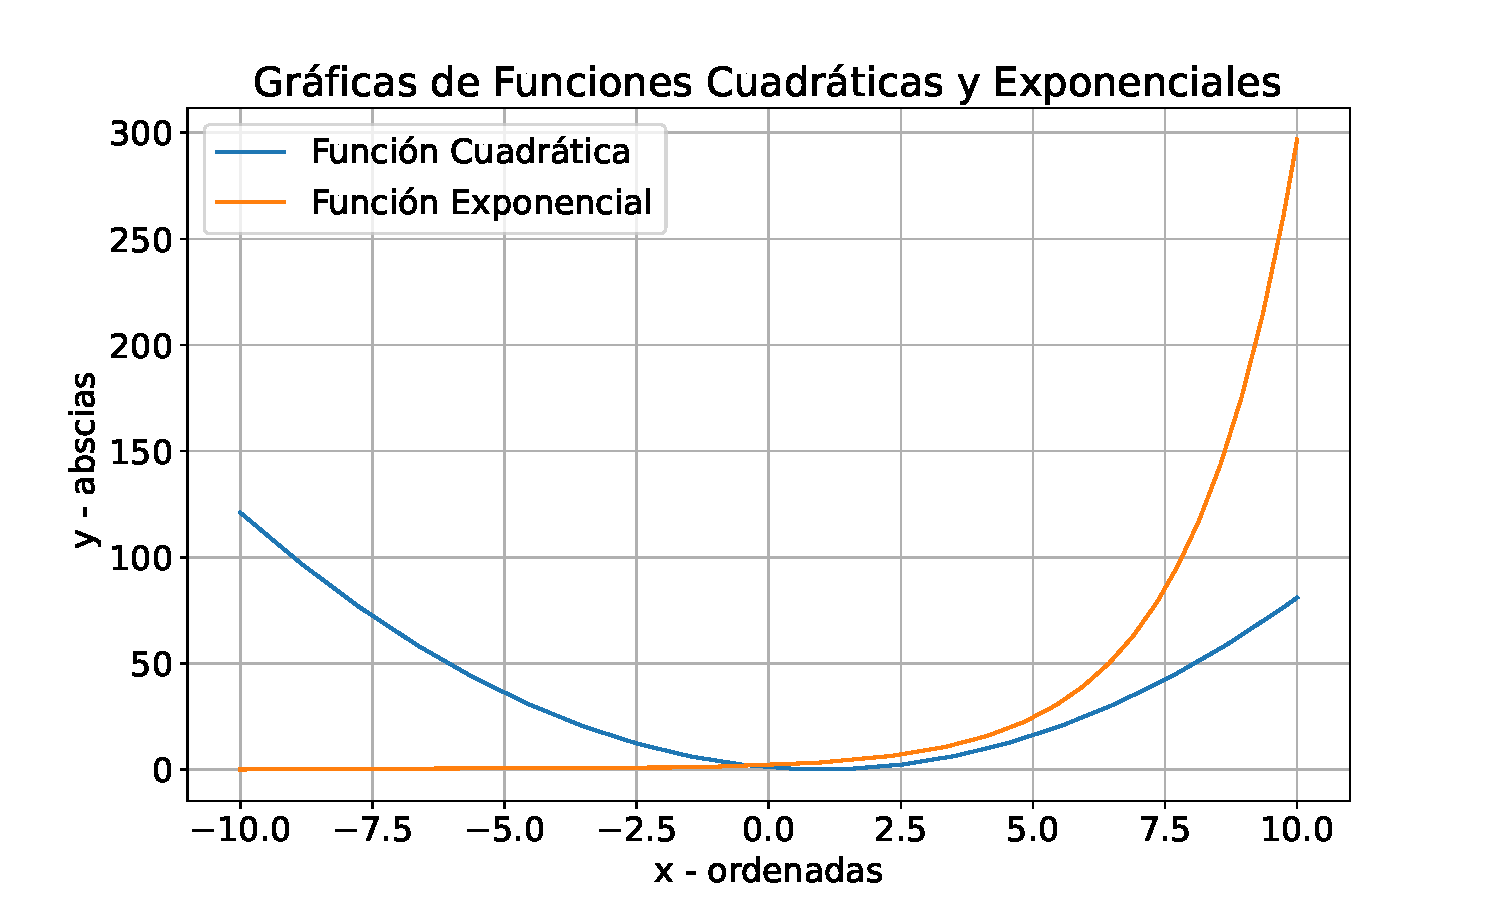
\includegraphics[scale=0.3]{exp}
            \captionof{figure}{Se observa la regla principal y nonius del que compone el Calibrador Vernier o pie de rey.}
        \end{center}
        \noindent La figura 1 muestra un esquema para la lectura correcta en el nonius del Calibrador vernier.

        \subsection{\textbf{\textcolor{magenta}{Datos Experimentales}}}
        \noindent En esta sección va la Tabla de valores medidos u obtenidos mediante un instrumento de medición. En esta sección se presentan de forma organizada los datos obtenidos en el laboratorio, es importante utilizar el número correcto de cifras significativas, el número de cifras significativas dependerá de la precisión del instrumento utilizado para hacer las medidas por ejemplo:

        \begin{center}
            \begin{tabular}{|c||c|c|}
                \hline
                N  & D[mm] & E[mm] \\[0,1cm]
                \hline \hline
                1  &       &       \\ \hline
                2  &       &       \\ \hline
                3  &       &       \\ \hline
                4  &       &       \\ \hline
                5  &       &       \\ \hline
                6  &       &       \\ \hline
                7  &       &       \\ \hline
                8  &       &       \\ \hline
                9  &       &       \\ \hline
                10 &       &       \\ \hline
            \end{tabular}
        \end{center}
        Tabla 1. Se muestra en la tabla los valores experimentales medidos a partir de un Calibrador Vernier.


        \section{\textbf{\textcolor{red}{Resultados y análisis}}}
        \noindent Presente los resultados en el orden en que fueron calculados y obtenidos, de manera organizada. Por lo general se utilizan tablas cuando los cálculos son repetitivos para una o más variables independientes. Todas las tablas y figuras deben tener un número de referencia. La discusión es la parte más importante del Informe de Laboratorio ya que en ella el estudiante demuestra que tiene dominio del experimento realizado y de los principios en los cuales éste está basado. En la discusión no sólo se analizan los resultados sino que se discute las implicaciones de los mismos.


        \section{\textbf{\textcolor{blue}{Conclusiones}}}
        \noindent En esta sección se resumen brevemente los aspectos más importantes de los objetivos del experimento. Además se discute brevemente la importancia del experimento. Se muestra hasta que punto se ha cumplido los objetivos. Se respaldan las afirmaciones con evidencia lógica, o referencias específicas de la literatura. Se establece claramente lo que se ha logrado, junto con el error relativo porcentual asociado a los resultados. En esta sección se puede también criticar el experimento y hacer recomendaciones para mejorarlo.


        \section{\textbf{\textcolor{red}{Referencias bibliográficas}}}
        \noindent Se debe incluir en esta sección los textos, artículos de publicaciones científicas nacionales o extranjeras, paginas web u otras, utilizadas en el informe, estos deben ir numerados y en orden alfabético -debe ir primero el autor principal y luego los otros autores, año de publicación, titulo del texto (si corresponde), título del artículo, mencionar la editorial (en caso de textos), editorial donde se publicó el artículo. \\
        \begin{thebibliography}{10}
            \bibitem{1} D. C. Baird (1995). Experimentación: Una introducción a la teoría de mediciones y al diseño de experimentos (2da Ed.) Mexico: Prentice-Hall Hispanoamericana.
            \bibitem{2} Alvarez, A. C. y Huayta, E. C. (2008). Medidas y Errores (3ra Ed.) La Paz - Bolivia: Catacora.

            \bibitem{3} http://www.scielo.org.mx/pdf/rmfe/v58n1/
            \bibitem{4} https://www.fuerzaycontrol.com/la-velocidad-de-reaccion-el-tiempo-de-reaccion-simple-complejo-la-anticipacion/
            \bibitem{5} https://www.redalyc.org/pdf/2742/274222159010.pdf
            \bibitem{6} https://brainly.lat/tarea/12199656
            \bibitem{7} https://chat.openai.com/
            \bibitem{8} https://www.bbc.com/mundo/noticias-45760025
            \bibitem{9} https://www.cognifit.com/bo/tiempo-de-respuesta.
            % fuentes pregunta 3
            \bibitem{10} CogniFit. (s. f.). Tiempo De Reacción o Tiempo de Respuesta - Habilidad Cognitiva. https://www.cognifit.com/es/tiempo-de-respuesta
            \bibitem{11} Pérez, C. (s. f.). cuál es la importancia del tiempo de respuesta? prezi.com. https://prezi.com/r3jhafg7mcc7/cual-es-la-importancia-del-tiempo-de-respuesta
            \bibitem{12} Univision. (s. f.). ¿Por qué el tiempo de reacción es CLAVE y cómo influye en nuestro día a día? Univision. https://www.univision.com/explora/por-que-el-tiempo-de-reaccion-es-clave-y-como-influye-en-nuestro-dia-a-dia
            \bibitem{13} Team, V. (2023). Tiempo de reacción, entrenamiento para mejorarlo. Vitruve | Velocity-Based Training. https://vitruve.fit/es/blog/tiempo-de-reaccion-entrenamiento-para-mejorarlo/
            % fuentes pregunta 4
            \bibitem{14} Facultad de Ciencias de la Actividad Física y del Deporte (INEF)(UPM). (s. f.). Estudio del tiempo de reacción ante estímulos sonoros y visuales. - Archivo Digital UPM. https://oa.upm.es/12070/
            \bibitem{15} Estudio del tiempo de reacción ante estímulos sonoros y visuales. (s. f.). Grupo Sobre Entrenamiento (G-SE). https://g-se.com/estudio-del-tiempo-de-reaccion-ante-estimulos-sonoros-y-visuales-bp-V57cfb26ec18eb


        \end{thebibliography}
    \end{multicols}
\end{document}
